% answers.tex —— 1977 年·江苏卷 · 参考答案与详细解析片段
% 由 tools/generate_projects.py 依来源总账自 1977/1977_数学真题_江苏_试题.md + 1977/1977_数学真题_江苏_解析正文.md + 1977/1977_数学真题_江苏_答案要点.md 生成，勿手改（改源 MD 后重跑）


\begin{gktip}
固定源为 A3 单页题面，未附答案页。第 1(1) 与附加题 7 的源面疑点按原样保留；下文明确区分“严格按题面”的结论和在常见排印误写假设下的候选结论。
\end{gktip}

\begin{answer}
\gksolhead{1}{}

\textbf{题目}：

解答下列各题：

\Needspace{5\baselineskip}
（1） 计算：

\nopagebreak[4]
\[
\left(2\frac14\right)^{\frac12}+\left(\frac1{10}\right)^{-2}-(3.14)^0+\left(-\frac{27}{8}\right)^{-\frac12}
\]

\Needspace{5\baselineskip}
（2） 求函数

\nopagebreak[4]
\[
y=\sqrt{x-2}+\frac1{x-3}+\lg(5-x)
\]

的定义域。

\Needspace{5\baselineskip}
（3） 解方程：

\nopagebreak[4]
\[
5^{x^2+2x}=125
\]

\Needspace{5\baselineskip}
（4） 计算：

\nopagebreak[4]
\[
-\log_3\left(\log_3\sqrt[3]{\sqrt[3]{\sqrt[3]{3}}}\right)
\]

\Needspace{5\baselineskip}
（5） 把直角坐标方程

\nopagebreak[4]
\[
(x-3)^2+y^2=9
\]

化为极坐标方程。

\Needspace{5\baselineskip}
（6） 计算：

\nopagebreak[4]
\[
\lim_{n\to\infty}\frac{1+2+3+\cdots+n}{n^2}
\]

\Needspace{5\baselineskip}
（7） 分解因式：

\nopagebreak[4]
\[
x^4-2x^2y-3y^2+8y-4
\]

\Needspace{4\baselineskip}
\textbf{解析}

\gksubpart{（1）}

\Needspace{5\baselineskip}
前两项及第三项为

\nopagebreak[4]
\[
\left(2\frac14\right)^{1/2}=\frac32,
\qquad
\left(\frac1{10}\right)^{-2}=100,
\qquad
(3.14)^0=1
\]

但 $-27/8$ 的 $-1/2$ 次幂在实数范围内没有定义。因此严格按固定源题面，整个式子没有实数值。不能把它擅自改成正数底数或其他指数。

\gksubpart{（2）}

\Needspace{5\baselineskip}
根式要求 $x-2\ge0$，对数要求 $5-x>0$，分式要求 $x\ne3$。合并得

\nopagebreak[4]
\[
x\ge2,\qquad x<5,\qquad x\ne3
\]

\Needspace{5\baselineskip}
所以定义域为

\nopagebreak[4]
\[
[2,3)\cup(3,5)
\]

\gksubpart{（3）}

\Needspace{5\baselineskip}
因为 $125=5^3$ 且底数 $5>0$ 且 $5\ne1$，所以

\nopagebreak[4]
\[
x^2+2x=3
\quad\Longleftrightarrow\quad
x^2+2x-3=0
\quad\Longleftrightarrow\quad
(x-1)(x+3)=0
\]

故 $x=1$ 或 $x=-3$。

\gksubpart{（4）}

\Needspace{5\baselineskip}
三重立方根为

\nopagebreak[4]
\[
\sqrt[3]{\sqrt[3]{\sqrt[3]{3}}}=3^{1/27}
\]

\Needspace{5\baselineskip}
于是内层对数为 $1/27$，外层对数为 $-3$，故

\nopagebreak[4]
\[
-\log_3\left(\log_3\sqrt[3]{\sqrt[3]{\sqrt[3]{3}}}\right)=3
\]

\gksubpart{（5）}

\Needspace{5\baselineskip}
令 $x=r\cos\theta$、$y=r\sin\theta$，则

\nopagebreak[4]
\[
(r\cos\theta-3)^2+r^2\sin^2\theta=9
\]

\Needspace{5\baselineskip}
化简得

\nopagebreak[4]
\[
r^2-6r\cos\theta=0
\]

\Needspace{5\baselineskip}
所以极坐标方程可写为

\nopagebreak[4]
\[
r=6\cos\theta
\]

\gksubpart{（6）}

\Needspace{5\baselineskip}
利用等差数列求和公式，

\nopagebreak[4]
\[
\frac{1+2+\cdots+n}{n^2}
=\frac{n(n+1)}{2n^2}
=\frac{n+1}{2n}
\longrightarrow\frac12
\]

\gksubpart{（7）}

\Needspace{5\baselineskip}
把 $x^2$ 暂作一个整体，配合交叉项可得

\nopagebreak[4]
\[
\begin{aligned}
x^4-2x^2y-3y^2+8y-4
&=(x^2-3y+2)(x^2+y-2)
\end{aligned}
\]

\gkanswer{答案（1）：严格按题面，$(-27/8)^{-1/2}$ 在实数范围内无定义，故原式无实数值。}

\gkanswer{答案（2）：$[2,3)\cup(3,5)$。}

\gkanswer{答案（3）：$x=1$ 或 $x=-3$。}

\gkanswer{答案（4）：$3$。}

\gkanswer{答案（5）：$r=6\cos\theta$。}

\gkanswer{答案（6）：$\dfrac12$。}

\gkanswer{答案（7）：$(x^2-3y+2)(x^2+y-2)$。}

\end{answer}
\begin{answer}
\gksolhead{2}{}

\textbf{题目}：

过抛物线 $y^2=4x$ 的焦点作倾斜角为 $\dfrac{3\pi}{4}$ 的直线，它与抛物线相交于 $A\text{、}B$ 两点。求 $A\text{、}B$ 两点间的距离。

\Needspace{4\baselineskip}
\textbf{解析}

\Needspace{5\baselineskip}
抛物线 $y^2=4x$ 的焦点为 $(1,0)$。倾斜角为 $3\pi/4$ 的直线斜率为 $-1$，故直线方程为

\nopagebreak[4]
\[
y=-(x-1)=-x+1
\]

\Needspace{5\baselineskip}
与抛物线联立：

\nopagebreak[4]
\[
(1-x)^2=4x
\quad\Longleftrightarrow\quad
x^2-6x+1=0
\]

\Needspace{5\baselineskip}
所以交点的横坐标为 $x_1=3-2\sqrt2$、$x_2=3+2\sqrt2$。两点在斜率为 $-1$ 的直线上，故

\nopagebreak[4]
\[
AB=\sqrt{(x_2-x_1)^2+(y_2-y_1)^2}
=\sqrt2\,(4\sqrt2)=8
\]

\gkanswer{答案：$AB=8$。}

\end{answer}
\begin{answer}
\gksolhead{3}{}

\textbf{题目}：

在直角三角形 $ABC$ 中，$\angle ACB=90^\circ$，$CD\text{、}CE$ 分别为斜边 $AB$ 上的高和中线，且 $\angle BCD$ 与 $\angle ACD$ 之比为 $3:1$，求证：$CD=DE$。
\nopagebreak[4]
\begin{center}% 1977 年江苏卷第 3 题：直角三角形中的高与中线
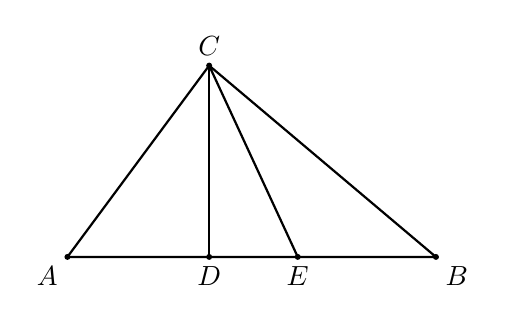
\begin{tikzpicture}[scale=0.9]
  \coordinate (A) at (0,0);
  \coordinate (D) at (2.0,0);
  \coordinate (E) at (3.25,0);
  \coordinate (B) at (5.2,0);
  \coordinate (C) at (2.0,2.7);
  \draw[thick] (A)--(C)--(B)--cycle;
  \draw[thick] (C)--(D);
  \draw[thick] (C)--(E);
  \fill (A) circle (1.2pt) node[below left] {$A$};
  \fill (B) circle (1.2pt) node[below right] {$B$};
  \fill (C) circle (1.2pt) node[above] {$C$};
  \fill (D) circle (1.2pt) node[below] {$D$};
  \fill (E) circle (1.2pt) node[below] {$E$};
\end{tikzpicture}
\end{center}
\nopagebreak[4]
\Needspace{4\baselineskip}
\textbf{解析}

\Needspace{5\baselineskip}
设 $\angle ACD=\alpha$，则由 $CD\perp AB$，有 $\angle BCD=3\alpha$ 且

\nopagebreak[4]
\[
\alpha+3\alpha=90^\circ,
\qquad \alpha=22.5^\circ
\]

\Needspace{5\baselineskip}
在直角三角形 $ACD$、$BCD$ 中，取 $CD$ 为单位长度，则

\nopagebreak[4]
\[
AD=\cot22.5^\circ=\sqrt2+1,
\qquad
DB=\cot67.5^\circ=\sqrt2-1
\]

\Needspace{5\baselineskip}
从而

\nopagebreak[4]
\[
AB=AD+DB=2\sqrt2
\]

\Needspace{5\baselineskip}
而 $E$ 是 $AB$ 的中点，故 $AE=\sqrt2$，于是

\nopagebreak[4]
\[
DE=AD-AE=(\sqrt2+1)-\sqrt2=1=CD
\]

故 $CD=DE$。

\gkanswer{答案：见解析版。}

\end{answer}
\begin{answer}
\gksolhead{4}{}

\textbf{题目}：

在周长为 $300\ \mathrm{cm}$ 的圆周上，有甲、乙两球以大小不等的速度作匀速圆周运动。甲球从 $A$ 点出发按逆时针方向运动，乙球从 $B$ 点出发按顺时针方向运动，两球相遇于 $C$ 点；相遇后，两球各自反方向作匀速圆周运动，但这时甲球速度的大小是原来的 2 倍，乙球速度的大小是原来的一半，以后他们第二次相遇于 $D$ 点。已知弧 $\overset{\frown}{AmC}=40\ \mathrm{cm}$，弧 $\overset{\frown}{BnD}=20\ \mathrm{cm}$，求弧 $\overset{\frown}{ACB}$ 的长度。

\Needspace{4\baselineskip}
\textbf{解析}

设圆周长为 $L=300\ \mathrm{cm}$，以甲球从 $A$ 出发的逆时针方向为正方向。第一次相遇时，甲球从 $A$ 到 $C$ 的路程为题给弧长 $40\ \mathrm{cm}$。设从 $C$ 沿逆时针方向到 $B$ 的弧长为 $q$，则所求弧 $\overset{\frown}{ACB}$ 的长度为 $40+q$。

\Needspace{5\baselineskip}
第一次相遇给出初速度比

\nopagebreak[4]
\[
\frac{u}{v}=\frac{40}{q}
\]

\Needspace{5\baselineskip}
相遇后甲球反向以 $2u$ 运动，乙球反向以 $v/2$ 运动。它们从 $C$ 向相反方向再次相遇，因此两段路程之和为 $L$。乙球从 $C$ 沿逆时针方向走到 $D$ 的距离为

\nopagebreak[4]
\[
d=\frac{L(v/2)}{2u+v/2}=\frac{Lq}{q+160}
\]

\Needspace{5\baselineskip}
题给弧 $\overset{\frown}{BnD}=20\ \mathrm{cm}$，故 $d-q=20$。代入 $L=300$：

\nopagebreak[4]
\[
\frac{300q}{q+160}-q=20
\quad\Longleftrightarrow\quad
q^2-120q+3200=0
\]

\Needspace{5\baselineskip}
解得 $q=40$ 或 $q=80$。题面说明两球初速度大小不等，而 $q=40$ 时 $u/v=1$，应舍去；故 $q=80$。因此

\nopagebreak[4]
\[
\overset{\frown}{ACB}=40+80=120\ \mathrm{cm}
\]

\gkanswer{答案：弧 $\overset{\frown}{ACB}=120\ \mathrm{cm}$。}

\end{answer}
\begin{answer}
\gksolhead{5}{}

\textbf{题目}：

（1） 若三角形三内角成等差数列，求证：必有一内角为 $60^\circ$。

（2） 若三角形三内角成等差数列，而且三边又成等比数列，求证：三角形三内角都是 $60^\circ$。

\Needspace{4\baselineskip}
\textbf{解析}

\gksubpart{（1）}

设三个内角按递增顺序为 $60^\circ-\alpha$、$60^\circ$、$60^\circ+\alpha$。这是因为三个内角的和为 $180^\circ$，等差数列的中项等于平均数。因此必有一个内角为 $60^\circ$。

\gksubpart{（2）}

\Needspace{5\baselineskip}
由正弦定理，三边与三个内角的正弦成正比。三边成等比数列意味着中间一边的平方等于两边之积，于是

\nopagebreak[4]
\[
\sin^260^\circ=\sin(60^\circ-\alpha)\sin(60^\circ+\alpha)
\]

利用积化和差公式，右端为 $\sin^260^\circ-\sin^2\alpha$，故 $\sin\alpha=0$。三角形内角范围迫使 $\alpha=0$，所以三个内角均为 $60^\circ$。

\gkanswer{答案（1）：见解析版；其中一个内角为 $60^\circ$。}

\gkanswer{答案（2）：三个内角均为 $60^\circ$。}

\end{answer}
\begin{answer}
\gksolhead{6}{}

\textbf{题目}：

在两条平行直线 $AB$ 和 $CD$ 上分别取定一点 $M$ 和 $N$，在线段 $AB$ 上取一定线段 $ME=a$；在线段 $MN$ 上取一点 $K$，连结 $EK$ 并延长交 $CD$ 于 $F$。试问 $K$ 取在哪里时，$\triangle EMK$ 与 $\triangle FNK$ 的面积之和最小？最小值是多少？

\begin{gktip}
\Needspace{0.25\textheight}
\textbf{附加题}
\end{gktip}

\Needspace{5\baselineskip}
\textbf{附加题 7．} 求极限：

\nopagebreak[4]
\[
\lim_{n\to\infty}\sqrt{x}\left(\sqrt{x+1}-\sqrt{x}\right)
\]

\Needspace{5\baselineskip}
\textbf{附加题 8．} 求不定积分：

\nopagebreak[4]
\[
\int\frac{\mathrm dx}{(1+\mathrm e^x)^2}
\]

\Needspace{4\baselineskip}
\textbf{解析}

\Needspace{5\baselineskip}
设两平行直线的距离为 $h$，令

\nopagebreak[4]
\[
t=\frac{MK}{MN},\qquad 0<t<1
\]

\Needspace{5\baselineskip}
由相似三角形，$K$ 到两平行线的距离分别为 $th$、$(1-t)h$，并且

\nopagebreak[4]
\[
FN=ME\frac{KN}{MK}=a\frac{1-t}{t}
\]

\Needspace{5\baselineskip}
因此两个三角形面积之和为

\nopagebreak[4]
\[
\begin{aligned}
S(t)&=\frac12a(th)+\frac12\left(a\frac{1-t}{t}\right)((1-t)h)\\
&=\frac{ah}{2}\left(2t+\frac1t-2\right)
\end{aligned}
\]

\Needspace{5\baselineskip}
由 $2t+1/t\ge2\sqrt2$，当且仅当 $t=1/\sqrt2$ 时取等号。因此

\nopagebreak[4]
\[
\frac{MK}{MN}=\frac1{\sqrt2},
\qquad
S_{\min}=ah(\sqrt2-1)
\]

\gksubpart{附加题 7}

\Needspace{4\baselineskip}
\textbf{解析}

\Needspace{5\baselineskip}
固定源题面写作

\nopagebreak[4]
\[
\lim_{n\to\infty}\sqrt{x}\left(\sqrt{x+1}-\sqrt{x}\right)
\]

表达式只含 $x$，没有说明 $x$ 如何随 $n$ 变化，因此按字面它不是一个可由 $n\to\infty$ 唯一确定的数值极限。

\Needspace{5\baselineskip}
若按常见排印误写将两个 $x$ 都理解为 $n$，则

\nopagebreak[4]
\[
\begin{aligned}
\sqrt n(\sqrt{n+1}-\sqrt n)
&=\sqrt n\frac1{\sqrt{n+1}+\sqrt n}\\
&=\frac1{\sqrt{1+1/n}+1}\longrightarrow\frac12
\end{aligned}
\]

该 $1/2$ 只能作为“$x$ 应为 $n$”假设下的候选答案。

\gksubpart{附加题 8}

\Needspace{4\baselineskip}
\textbf{解析}

\Needspace{5\baselineskip}
令 $t=\mathrm e^x$，则 $\mathrm dx=\mathrm dt/t$，有

\nopagebreak[4]
\[
\frac1{t(1+t)^2}=\frac1t-\frac1{1+t}-\frac1{(1+t)^2}
\]

\Needspace{5\baselineskip}
所以

\nopagebreak[4]
\[
\begin{aligned}
\int\frac{\mathrm dx}{(1+\mathrm e^x)^2}
&=\int\left(\frac1t-\frac1{1+t}-\frac1{(1+t)^2}\right)\mathrm dt\\
&=\ln t-\ln(1+t)+\frac1{1+t}+C\\
&=x-\ln(1+\mathrm e^x)+\frac1{1+\mathrm e^x}+C
\end{aligned}
\]

\gkanswer{答案：设两平行直线的距离为 $h$，则当 $\dfrac{MK}{MN}=\dfrac1{\sqrt2}$ 时面积和最小，最小值为 $ah(\sqrt2-1)$。}

\end{answer}